\section{Transform Coding and JPEG}




\begin{questionbox}{Domanda 18}
Why the geometric mean of the variances of a random vector is key information to evaluate the \textbf{\textbf{rate}-\textbf{distortion}} performance of a \textbf{quantizer}?
\end{questionbox}


With high-resolution \textbf{quantization} and optimal \textbf{bit allocation}, the \textbf{distortion} after transform coding is proportional to the geometric mean of transformed coefficient variances:


$$
D^\star = c_{GM}\sigma_{GM}^2 2^{-2\bar{R}}
$$


Orthogonal transforms preserve total energy, hence preserve the arithmetic mean of variances:


$$
\sigma_{AM,Y}^2 = \sigma_{AM,X}^2
$$


but they can change the distribution of variances. A good transform makes few coefficients high-energy and many coefficients low-energy, reducing $\sigma_{GM}^2$. Since:


$$
\sigma_{GM}^2 \le \sigma_{AM}^2
$$


smaller geometric mean means lower \textbf{distortion} at the same \textbf{rate}.

Coding gain is:


$$
G_T = \frac{D_{\text{PCM}}}{D_Y}
=\frac{\sigma_{AM,Y}^2}{\sigma_{GM,Y}^2}
$$


and in dB:


$$
G_{T,dB}=10\log_{10}G_T
$$




\begin{questionbox}{Domanda 19}
Write the resource allocation problem for transform coding. Derive the Huang-Schulteiss formula.
\end{questionbox}


For a vector with components $k=0,\dots,M-1$, high-resolution \textbf{distortion} is:


$$
D = \frac{1}{M}\sum_{k=0}^{M-1} c_k\sigma_k^2 2^{-2R_k}
$$


subject to:


$$
\sum_{k=0}^{M-1} R_k \le R_{\text{tot}}
$$


Lagrangian:


$$
J(\vec{R},\lambda)=
\frac{1}{M}\sum_{k=0}^{M-1} c_k\sigma_k^2 2^{-2R_k}
+\lambda\left(\sum_{k=0}^{M-1}R_k-R_{\text{tot}}\right)
$$


Set:


$$
\frac{\partial J}{\partial R_k}=0
$$


This gives:


$$
R_k^\star = \frac{R_{\text{tot}}}{M}
+\frac{1}{2}\log_2\left(
\frac{c_k\sigma_k^2}{c_{GM}\sigma_{GM}^2}
\right)
$$


where:


$$
c_{GM}=\sqrt[M]{\prod_{k=0}^{M-1} c_k},
\quad
\sigma_{GM}^2=\sqrt[M]{\prod_{k=0}^{M-1}\sigma_k^2}
$$


Components above the geometric mean receive more bits; components below it receive fewer bits.



\begin{questionbox}{Domanda 20}
Explain why the \textbf{KLT} is the optimal linear transform for decorrelation and why the \textbf{DCT} is used in practice instead.
\end{questionbox}


The \textbf{Karhunen-Loeve Transform} is built from the eigenvectors of the signal covariance matrix. In that basis, transform coefficients are decorrelated and energy compaction is optimal among linear orthogonal transforms for the given source statistics.

If $R_X$ is the covariance matrix and $u_i$ are its eigenvectors, then:


$$
T_{KLT} = [u_1\ u_2\ \cdots\ u_M]^T
$$


The problem is that \textbf{KLT} depends on the actual statistics of the image or block. The encoder would need to estimate the covariance, compute the transform and signal it to the decoder.

The \textbf{DCT} is used in practice because it is fixed, separable, fast, \textbf{HAS} no side information cost and approximates the \textbf{KLT} well for locally correlated image blocks.



\begin{questionbox}{Domanda 21}
Describe the principles of the JPEG standard.
\end{questionbox}


JPEG is a \textbf{lossy} still-image coding standard based on block \textbf{DCT}, \textbf{quantization} and \textbf{entropy} coding. The standard mainly defines the decodable bitstream and decoder behavior, while encoder choices remain flexible.

Baseline JPEG chain:


\begin{figure}[H]
\centering
\begin{tikzpicture}[
    node distance=0.9cm,
    block/.style={draw, fill=blue!5, text width=5cm, align=center, minimum height=0.55cm, rounded corners=3pt, font=\small},
    arrow/.style={thick,->,>=stealth}
]
    \node (a) [block] {RGB};
    \node (b) [block, below=of a] {YCbCr};
    \node (c) [block, below=of b] {Chroma Subsampling};
    \node (d) [block, below=of c] {8x8 Blocks};
    \node (e) [block, below=of d] {Level Shift by 128};
    \node (f) [block, below=of e] {DCT};
    \node (g) [block, below=of f] {Quantization};
    \node (h) [block, below=of g] {Zig-zag Scan};
    \node (i) [block, below=of h] {RLE / Huffman};
    \node (j) [block, below=of i] {JPEG Bitstream};

    \draw [arrow] (a) -- (b);
    \draw [arrow] (b) -- (c);
    \draw [arrow] (c) -- (d);
    \draw [arrow] (d) -- (e);
    \draw [arrow] (e) -- (f);
    \draw [arrow] (f) -- (g);
    \draw [arrow] (g) -- (h);
    \draw [arrow] (h) -- (i);
    \draw [arrow] (i) -- (j);
\end{tikzpicture}
\caption{JPEG Baseline Encoding Chain}
\end{figure}


\textbf{quantization}:


$$
\tilde{C}_{ij}=\text{round}\left(\frac{C_{ij}}{q_{ij}}\right)
$$


The \textbf{quantization} table assigns different steps to \textbf{DCT} frequencies: smaller steps for visually important low frequencies, larger steps for high frequencies.

Quality factor scaling:


$$
S_F =
\begin{cases}
\frac{5000}{Q} & 1 \le Q \le 50\\
200-2Q & 50 < Q \le 99\\
1 & Q=100
\end{cases}
$$


The actual \textbf{quantization} table is scaled approximately as:


$$
q \leftarrow \frac{S_F}{100}q^\star
$$


JPEG metadata formats:

\begin{itemize}
  \item \textbf{JFIF:} interoperability metadata such as density, resolution and thumbnails.
  \item \textbf{EXIF:} camera metadata such as date/time, GPS and camera settings.
\end{itemize}



\begin{questionbox}{Domanda 22}
(TC\&JPEG) Draw the scheme and describe the functional blocks of a JPEG encoder.
\end{questionbox}


\begin{figure}[H]
\centering
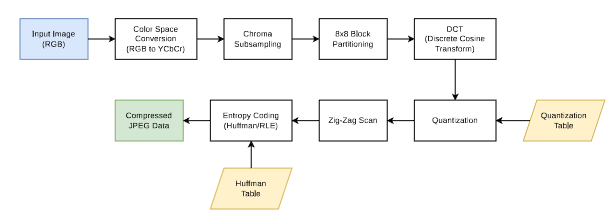
\includegraphics[width=0.75\textwidth]{images/JPEG_encoder.png}
\caption{JPEG encoder}
\end{figure}\begin{tcolorbox}[colback=white, colframe=gray!50, height=4.5cm, sharp corners]
\end{tcolorbox}

The \textbf{DCT} compacts energy; \textbf{quantization} creates losses; zig-zag scan groups zeros; \textbf{entropy} coding is \textbf{lossless}.



\begin{questionbox}{Domanda 23}
(TC\&JPEG) Describe the problem of “frequency leakage” in the Discrete Fourier Transform (DFT) when applied to signal compression and how the \textbf{discrete cosine transform} (\textbf{DCT}) addresses it.
\end{questionbox}


DFT assumes the finite signal is periodic. If the first and last samples do not match, periodization creates discontinuities. These discontinuities spread energy into high frequencies: this is frequency leakage.

\textbf{DCT} reduces leakage by using a symmetric extension of the signal before transforming it. The mirror boundary makes the periodic continuation smoother and improves energy compaction for images.



\begin{questionbox}{Domanda 24}
(TC\&JPEG) Explain the \textbf{entropy} coding process for AC coefficients in the JPEG standard and the significance of the “End of Block” (EOB) symbol.
\end{questionbox}


After zig-zag scan, AC coefficients are represented by pairs:


$$
(r,k)
$$


where:

\begin{itemize}
  \item $r$ is the run of preceding zeros.
  \item $k$ is the category of the non-zero coefficient amplitude.
\end{itemize}

Special symbols:


$$
(15,0) = \text{ZRL, run of 16 zeros}
$$



$$
(0,0) = \text{EOB, End Of Block}
$$


EOB means all remaining coefficients in the block are zero.



\begin{questionbox}{Domanda 25}
(TC\&JPEG) Describe the JPEG \textbf{lossless} coding process applied to the following table of quantized \textbf{DCT} coefficients:
\end{questionbox}

$$
> \begin{bmatrix}
> 10 & 3 & 0 & 0 & 0 & 0 & 0 & 0 \\
> -2 & 1 & 0 & 1 & 0 & 0 & 0 & 0 \\
> 1 & 0 & 0 & 0 & 0 & 0 & 0 & 0 \\
> 0 & 4 & 0 & 0 & 0 & 0 & 0 & 0 \\
> 0 & 0 & 0 & 0 & 0 & 0 & 0 & 0 \\
> 0 & 0 & 0 & 0 & 0 & 0 & 0 & 0 \\
> 0 & 0 & 0 & 0 & 0 & 0 & 0 & 0 \\
> 0 & 0 & 0 & 0 & 0 & 0 & 0 & 0
> \end{bmatrix}
> $$


Given the displayed coefficient matrix, treat missing positions as zero-padded to an $8\times 8$ block. The DC coefficient is:


$$
DC_n=10
$$


JPEG encodes the DC difference:


$$
\Delta DC = DC_n-DC_{n-1}
$$


If this is the first block and $DC_{n-1}=0$:


$$
\Delta DC=10
$$


The non-zero AC values in zig-zag order are:


$$
3,\ -2,\ 1,\ 1,\ 4,\ 1
$$


Run/category representation:


\begin{center}
\begin{tabular}{ | r | r | r | }
\hline
\textbf{AC value} & \textbf{Zero run} & \textbf{Category} \\
\hline
3 & 0 & 2 \\
\hline
-2 & 0 & 2 \\
\hline
1 & 0 & 1 \\
\hline
1 & 0 & 1 \\
\hline
4 & 6 & 3 \\
\hline
1 & 1 & 1 \\
\hline
EOB & 0 & 0 \\
\hline
\end{tabular}
\end{center}
No ZRL symbol is needed because there is no run longer than 15 zeros before a non-zero coefficient.



\begin{questionbox}{Domanda 26}
(TC\&JPEG) What is the primary purpose of an orthogonal transform in the context of the transform coding paradigm?
\end{questionbox}


The primary purpose of an orthogonal transform in transform coding is \textbf{sparsification / energy compaction}. It concentrates information into fewer coefficients while preserving energy and squared error:


$$
T^{-1}=T^T,\quad \|TX\|^2=\|X\|^2
$$




\begin{questionbox}{Domanda 27}
(TC\&JPEG) In the context of JPEG compression, what is the role of the \textbf{quantization} table?
\end{questionbox}


The \textbf{quantization} table defines the \textbf{quantization} step for each \textbf{DCT} coefficient. It controls \textbf{rate}-quality tradeoff and reflects visual sensitivity: low-frequency coefficients usually receive smaller steps than high-frequency coefficients.



\begin{questionbox}{Domanda 28}
(TC\&JPEG) Which statement regarding the relationship between the Arithmetic Mean (AM) and Geometric Mean (GM) of variances in transform coding is correct?
\end{questionbox}


Orthogonal transforms preserve energy, hence they preserve the arithmetic mean of coefficient variances. They do not necessarily preserve the geometric mean. Transform coding tries to reduce the GM while keeping the AM fixed, because optimal \textbf{distortion} depends on the GM.

---


